\section{Introduction}
\label{sec:introduction}

The \ac{GP} is a well-known tool in machine learning for performing nonparametric Bayesian
inference and learning.  The primary concern for it's adaptation for large regression
problems is its time and memory complexities of $O(n^3)$ and $O(n^2)$, respectively.  To
overcome this limitation, researchers have explored the use of sparsity in \ac{GP}
regression~\cite{lawrence2002fast,seeger2003fast,smola2001sparse,williams2001using}.  This
report aims to use parallelism, in addition to sparsity, to implement \ac{GP} regression
for large datasets.

In~\cite{keane2002data}, they partitioned the data into disjoint subsets using their
``GeoClust'' clustering algorithm, and learned a \ac{GP} for each subset.  Though they
reported good load balancing, there are actually a number of problems with GeoClust for
general datasets.  The algorithm assumes that the training features are uniformly
distributed in an $n$-dimensional hypercube.  When this is not the case, the algorithm
produces undefined cluster centers, where some \acp{PE} are assigned either very little
data or none at all, making their parallel \ac{GP} implementation very inefficient.  This
behavior is shown in Figure~\ref{fig:geoclust}.  Furthermore, even with perfect load
balancing,GeoClust is still an approximation to the full regression problem because
significant amounts of data are discarded for each cluster.

Instead of partitioning data into clusters, some researchers acheive parallelism by
randomly subsampling the training data.  In~\cite{chandola2011implementing}, they used a
mixed implementation of UNIX pthreads and the \ac{MPI} library to learn the \ac{GP}
hyperparameters over millions of timeseries.  In their implementation, the likelihood
gradient descent is done in parallel with one \ac{PE} per timeseries.  Though their
speedup is linear, their results are still an approximation because each timeseries is
learned separately.  Finally, it should be mentioned that in terms of parallelism, both of
the approaches in ~\cite{keane2002data, chandola2011implementing} are only slightly more
involved than ``embarrassingly parallel'' because not more than one \ac{PE} may run on a
given timeseries or partition of training data.

This report is based heavily on the preliminary theory and results
from~\cite{melkumyan2009sparse}, in which they derive two classes of exactly-sparse
covariance functions with a number of interesting properties.  First of all, this kernel
is sparse unlike the commonly-used radial basis kernels which result in 100\% dense
covariance matrices.  Further, the kernels derived in~\cite{melkumyan2009sparse} are
continuous and have continuous derivatives.  This nice property implies that the posterior
distribution is smooth unlike the aforementioned approximate methods which would result in
a posterior with many discontinuities.

For the experiments in~\cite{melkumyan2009sparse}, it was not clear how well the approach
scales for very large problems.  The datasets from their paper consisted of no more than
5,000 training points, thus resulting in solving a 5,000$\times$5,000 linear system.  A
problem of this size is considered somewhat small in modern parallel computing.  The
authors also mention using the Matlab sparse matrix package, which is typically used in
conjunction with direct factorization methods like Cholesky decomposition to solve linear
systems.  Though this approach is appropriate for small problems, we wanted to explore the
\ac{GP} on very large problems for the EECS 587 project.

\begin{figure}[t]
  \begin{center}
    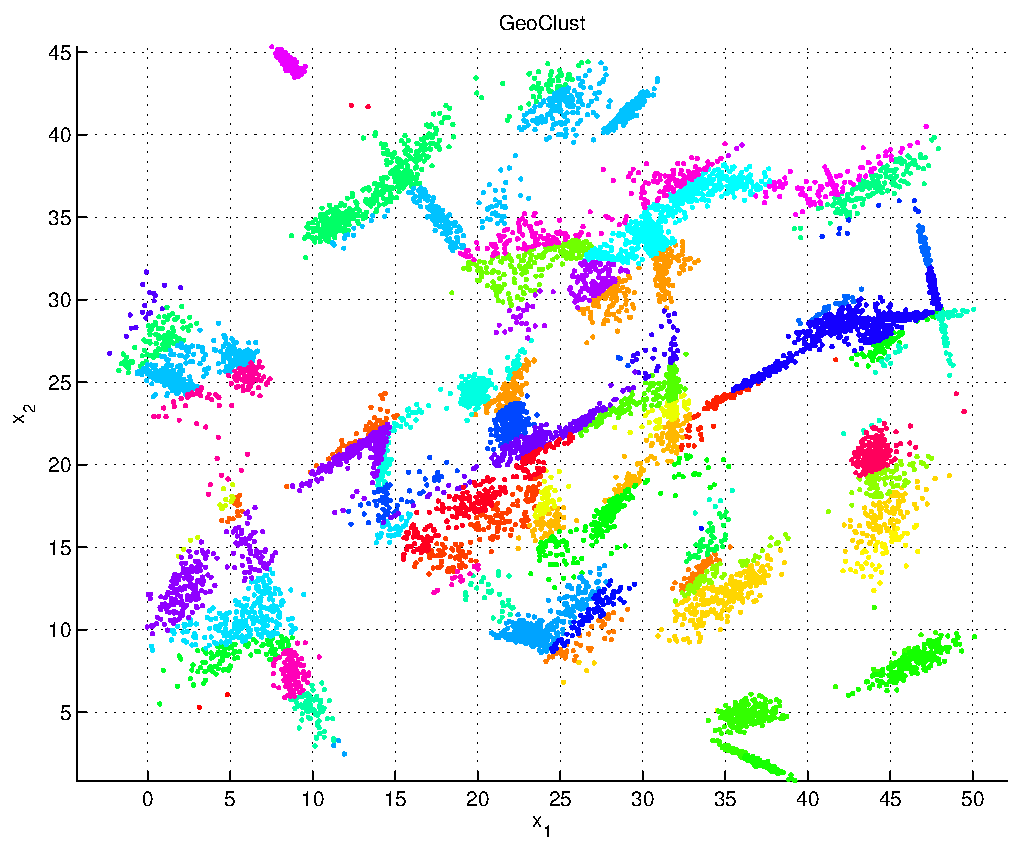
\includegraphics[width=.45\textwidth]{figures/geoclust}
    \caption{ {\small The ``GeoClust'' algorithm from~\cite{keane2002data} breaks when the
        data is not uniformly distributed in the space of features, as in this 2D example.
        The number of \acp{PE} is 50, but five \acp{PE} are not assigned any data at all.
        Of the 45 \acp{PE} that have data (denoted by different colors), the load balancing
        is poor. This project aims to avoid approximations based on clustering the
        training data altogether and instead focuses on parallel iterative solvers to
        improve performance.  } }
    \label{fig:geoclust}
  \end{center}
\end{figure}

This project aims to dive deeper into the performance of sparse kernels than what is
covered in~\cite{melkumyan2009sparse}, particularly for very large datasets.  In
\secref{sec:overviewofgaussianprocessregression}, we provide an overview of \ac{GP}
regression, and highlight the important considerations when done in a parallel
environment.  In \secref{sec:restatementofprojectgoals}, we concisely state the goals of
the project before going over our implementation in \secref{sec:implementation}.  Finally,
\secref{sec:experiments} covers the timing results of our algorithm.

%%% Local Variables: 
%%% mode: latex
%%% TeX-master: "../report.tex"
%%% End: 
